\section[Scattering Experiments (X-ray diffraction)]{\hyperlink{toc}{Scattering Experiments (X-ray diffraction)}}

~ Shining of wave on a crystal and detecting the scattered particles/radiation

- x-rays, electrons and neutrons

- wavelength of radiation should be comparable to a typical inter atomic distance of a few $\text{\AA}$.

\[E = h\nu = \frac{hc}{\lambda}\]

\[ \lambda(\text{\AA}) = 12398/E(eV)\]

- a few keV is needed for a wavelength of around 1 angstrom.

\textbf{X-Ray}
\begin{itemize}
    \item $\lambda = 1 \text{\AA}$
    \item E ~ $10^4 eV$
    \item interact with electron
    \item penetrating
\end{itemize}
\textbf{Neutron}
\begin{itemize}
    \item $\lambda = 1 \text{\AA}$
    \item E ~ $0.08 eV$
    \item interact with nuclei
    \item Highly penetrating
\end{itemize}
\textbf{Electron}
\begin{itemize}
    \item $\lambda = 2 \text{\AA}$
    \item E ~ $150 eV$
    \item interact with electron
    \item Less penetrating
\end{itemize}

- X-ray is great for bulk investigation
- Electron is great for surface investigation (checking surfaces with MBE)



\begin{tcolorbox}[enhanced,attach boxed title to top center={yshift=-3mm,yshifttext=-1mm},
  colback=blue!5!white,colframe=blue!75!black,colbacktitle=red!80!black,
  title=The Bragg Law,fonttitle=\bfseries,
  boxed title style={size=small,colframe=red!50!black} ]
  \begin{equation}
      2d\cdot\sin(\theta) = m\lambda 
  \end{equation}
\end{tcolorbox}

- Ignores some things but gives a good rough estimate with a simple model

- Diffraction occurs for:

\[ \vec{k} + \vec{G} = \vec{k}' \]

The larger the indices, the smaller the spacing between the planes.

- Single slit diffraction gives Fraunhover Diffraction Pattern
- This is a Fourier transform of the slit (or periodic crystal structure)

-   Atomic Form Factor increases with atomic charge.

- Some planes are absent in X-ray diffraction and some show:

The missing orders follow rules depending on which type of lattive it is -- 
\begin{itemize}
    \item \textbf{Simple Cubic (sc):} any (hkl)
    \item \textbf{Body-centred cubic (bcc):} h+k+l=even
    \item \textbf{Face-centred cubic (fcc):} h, k and l all odd or all even.
    
\end{itemize}
\begin{tabular}{ |p{3cm}||p{3cm}|p{3cm}|p{3cm}|  }
 \hline
 \multicolumn{4}{|c|}{\textbf{Lattice Type}} \\
 \hline
 Miller Indices & sc (P) & bcc (I) & fcc (F)\\
 \hline
 100 & Y & N & N\\
 110 & Y & Y & N\\
 111 & Y & N & Y\\
 200 & Y & Y & Y\\
 210 & Y & N & N\\
 211 & Y & Y & N\\
 220 & Y & Y & Y\\
 310 & Y & Y & N \\
 311 & Y & N & Y \\
 \hline
\end{tabular}

N = will not give a diffraction pattern for these planes (due to interference).
Y = will give ...

\textbf{X-Ray Diffraction (XRD) Methods:}
\begin{itemize}
    \item Laue: not that good
    \item Rotatin Crystal: meh
    \item Powder: to get lattice parameters, polycrystal (powdered), monochromatic beam, variable angle.
    \begin{itemize}
        \item Debye-Schenner cone
        \item beam comes through holes
    \end{itemize}
\end{itemize}


\textbf{XRD Procedure}
\begin{itemize}
    \item Measure angle 
    \item $d = \frac{\lambda}{2\sin\theta}$
    \item bigger angle gives smaller d
    \item small d corresponds to higher miller indices
    \item scale d's by the first one (get d=1 for first)
    \item scale all d by an clever choice of integer N
    \item $N = h^2 + k^2 + l^2 $
    \item {hkl}
    \item $a = d \sqrt{h^2 + k^2 + l^2}$ (hopefully getting the same a for all)
    \end{itemize}

\begin{tabular}{ |p{2cm}|p{3cm}|p{2cm}|p{1.5cm}|p{1.5cm}|p{1.5cm}|  }
 \hline
 \multicolumn{6}{|c|}{\textbf{Scattering Selection Rules}} \\
 \hline
{hkl} & $N=h^2+k^2+l^2$ & Multiplicity & sc (P) & bcc (I) & fcc (F)\\
 \hline
 100 & 1 & 6        & * &   &  \\
 110 & 2 & 12       & * & * &  \\
 111 & 3 & 8        & * &   & *\\
 200 & 4 & 6        & * & * & *\\
 210 & 5 & 24       & * &   &  \\
 211 & 6 & 24       & * & * &  \\
 --- & 7 & --       &   &   &  \\
 220 & 8 & 12       & * & * & *\\
 221,300 & 9 & 24+6 & * &   &  \\
 310 & 10 & 24      & * & * &  \\
 311 & 11 & 24      & * &   & *\\
 222 & 12 & 8       & * & * & *\\
 320 & 13 & 24      & * &   &  \\
 321 & 14 & 48      & * & * &  \\
 --- & 15 & --      &   &   &  \\
 400 & 16 & 6       & * & * & *\\
 \hline
\end{tabular}

\textbf{XRD Identification of SC,BCC, FCC:}
\begin{itemize}
    \item P (SC): N = 1,2,3,4,5,6,8,9,... (=all integers excluding 7,15,23,...)
    \item I (BCC): N = 2,4,6,8,10,12,14,... (=even integers excluding 28, 60,...)
    \item F (FCC): N = 3,4,8,11,12,16,19,20,...
\end{itemize}


\begin{figure}
  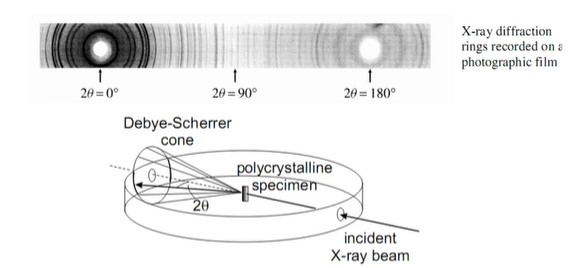
\includegraphics[width=0.75\linewidth]{Images/XRD.jpg}
  \caption{XRD}
  \label{fig:XRD}
\end{figure}
